\documentclass{atistandalonetask}
\usepackage{atistandard}
\begin{document}
  \begin{atiTask}[
    title = Die \textsc{Heaviside}sche Sprungfunktion
  ]
  
  Eine elektrische Ladung $Q$ sei gleichmäßig auf der $x$-Achse zwischen $x=-L/2$ und $x=L/2$ verteilt.
    \begin{atiSubtasks}
    	\item Schreiben Sie mit Hilfe der \textsc{Heaviside}schen Sprungfuntion die Linien- und die Raumladungsdichte dieser Ladungsverteilung in kartesischen Koordinaten auf.
    	\item Notieren Sie die Gestalt dieser Raumladungsdichte in Zylinderkoordinaten.
    \end{atiSubtasks}	
  \end{atiTask}
  \begin{atiSolution}
   	Lösung folgt
  	%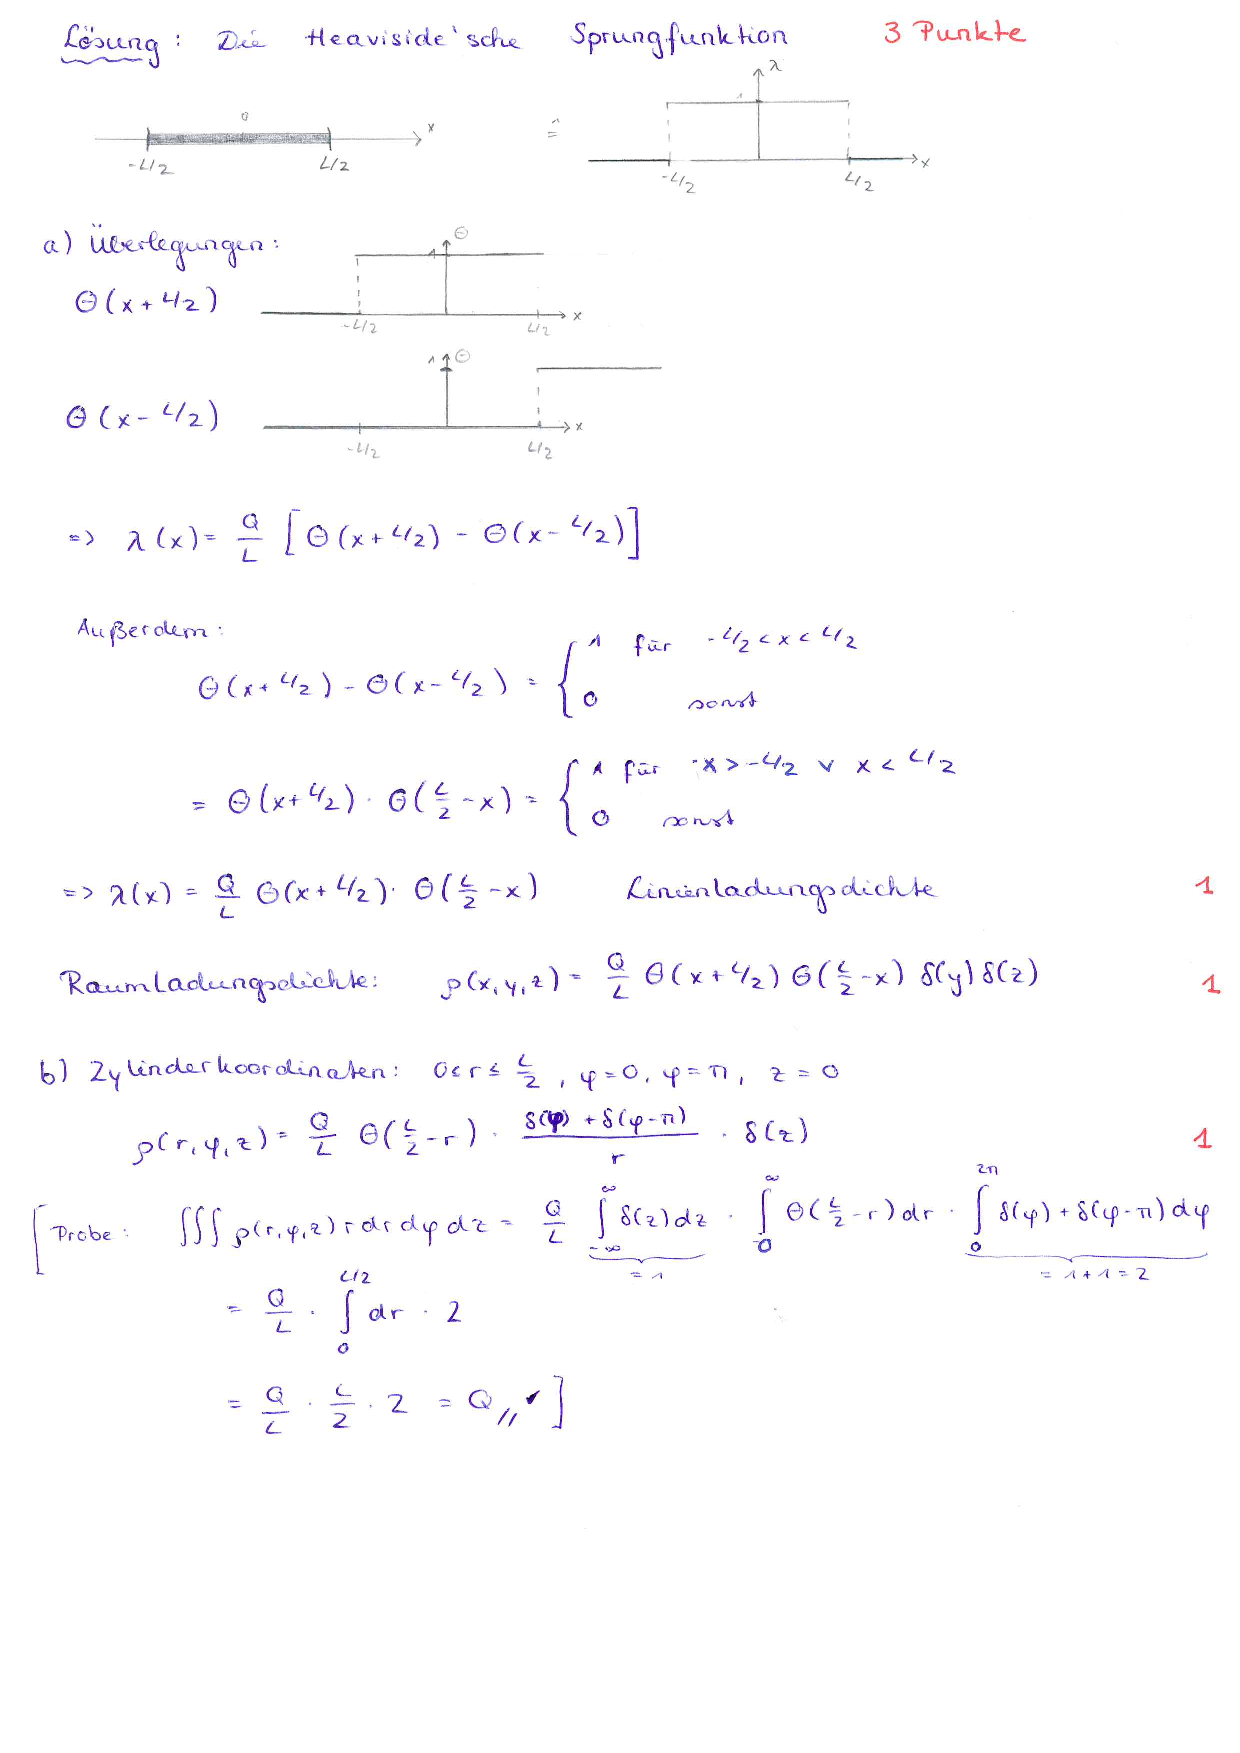
\includepdf[pages=-]{solution-heaviside_i.pdf}
  \end{atiSolution}
\end{document}